\documentclass[11pt,]{article}
\usepackage[left=1in,top=1in,right=1in,bottom=1in]{geometry}
\newcommand*{\authorfont}{\fontfamily{phv}\selectfont}
\usepackage[]{mathpazo}


  \usepackage[T1]{fontenc}
  \usepackage[utf8]{inputenc}




\usepackage{abstract}
\renewcommand{\abstractname}{}    % clear the title
\renewcommand{\absnamepos}{empty} % originally center

\renewenvironment{abstract}
 {{%
    \setlength{\leftmargin}{0mm}
    \setlength{\rightmargin}{\leftmargin}%
  }%
  \relax}
 {\endlist}

\makeatletter
\def\@maketitle{%
  \newpage
%  \null
%  \vskip 2em%
%  \begin{center}%
  \let \footnote \thanks
    {\fontsize{18}{20}\selectfont\raggedright  \setlength{\parindent}{0pt} \@title \par}%
}
%\fi
\makeatother




\setcounter{secnumdepth}{0}


\usepackage{graphicx,grffile}
\makeatletter
\def\maxwidth{\ifdim\Gin@nat@width>\linewidth\linewidth\else\Gin@nat@width\fi}
\def\maxheight{\ifdim\Gin@nat@height>\textheight\textheight\else\Gin@nat@height\fi}
\makeatother
% Scale images if necessary, so that they will not overflow the page
% margins by default, and it is still possible to overwrite the defaults
% using explicit options in \includegraphics[width, height, ...]{}
\setkeys{Gin}{width=\maxwidth,height=\maxheight,keepaspectratio}


\title{Patient's age prediction based on medical diagnosis of teeth
maturity \thanks{We would like to thanks the doctors who delivered their
experienced assesment of teeth maturity as well as our teacher who
provided us the data to work with.}  }
 



\author{\Large De La Torre
Camilo\vspace{0.05in} \newline\normalsize\emph{Universite Toulouse 1
Capitole}   \and \Large Campan
Alexis\vspace{0.05in} \newline\normalsize\emph{Universite Toulouse 1
Capitole}  }


\date{}

\usepackage{titlesec}

\titleformat*{\section}{\normalsize\bfseries}
\titleformat*{\subsection}{\normalsize\itshape}
\titleformat*{\subsubsection}{\normalsize\itshape}
\titleformat*{\paragraph}{\normalsize\itshape}
\titleformat*{\subparagraph}{\normalsize\itshape}



\usepackage{biblatex}

\addbibresource{master.bib}


\newtheorem{hypothesis}{Hypothesis}
\usepackage{setspace}


% set default figure placement to htbp
\makeatletter
\def\fps@figure{htbp}
\makeatother


% move the hyperref stuff down here, after header-includes, to allow for - \usepackage{hyperref}

\makeatletter
\@ifpackageloaded{hyperref}{}{%
\ifxetex
  \PassOptionsToPackage{hyphens}{url}\usepackage[setpagesize=false, % page size defined by xetex
              unicode=false, % unicode breaks when used with xetex
              xetex]{hyperref}
\else
  \PassOptionsToPackage{hyphens}{url}\usepackage[draft,unicode=true]{hyperref}
\fi
}

\@ifpackageloaded{color}{
    \PassOptionsToPackage{usenames,dvipsnames}{color}
}{%
    \usepackage[usenames,dvipsnames]{color}
}
\makeatother
\hypersetup{breaklinks=true,
            bookmarks=true,
            pdfauthor={De La Torre Camilo (Universite Toulouse 1
Capitole) and Campan Alexis (Universite Toulouse 1 Capitole)},
             pdfkeywords = {Teeth, Age, Regression, Machine Learning,
GBRT},  
            pdftitle={Patient's age prediction based on medical
diagnosis of teeth maturity},
            colorlinks=true,
            citecolor=blue,
            urlcolor=blue,
            linkcolor=magenta,
            pdfborder={0 0 0}}
\urlstyle{same}  % don't use monospace font for urls

% Add an option for endnotes. -----


% add tightlist ----------
\providecommand{\tightlist}{%
\setlength{\itemsep}{0pt}\setlength{\parskip}{0pt}}

% add some other packages ----------

% \usepackage{multicol}
% This should regulate where figures float
% See: https://tex.stackexchange.com/questions/2275/keeping-tables-figures-close-to-where-they-are-mentioned
\usepackage[section]{placeins}


\begin{document}
	
% \pagenumbering{arabic}% resets `page` counter to 1 
%    

% \maketitle

{% \usefont{T1}{pnc}{m}{n}
\setlength{\parindent}{0pt}
\thispagestyle{plain}
{\fontsize{18}{20}\selectfont\raggedright 
\maketitle  % title \par  

}

{
   \vskip 13.5pt\relax \normalsize\fontsize{11}{12} 
\textbf{\authorfont De La Torre
Camilo} \hskip 15pt \emph{\small Universite Toulouse 1
Capitole}   \par \textbf{\authorfont Campan
Alexis} \hskip 15pt \emph{\small Universite Toulouse 1 Capitole}   

}

}








\begin{abstract}

    \hbox{\vrule height .2pt width 39.14pc}

    \vskip 8.5pt % \small 

\noindent Our study involves patient's age prediction based on teeth
maturity that is assesed by doctors. Teeth are characterised by several
levels of maturity (going from A to H), data is often incomplete and for
some patients, teeth can't be evaluated because the patient does not
have them yet. After several attempts to mitigate the incompleteness of
our records, we obtained a very low Mean Absolute Error of 0.9 years in
predicting unseen data. The model that best generalized to unseen
records was a tuned GBRT (Gradient Boosting Regression Tree). Lastly, we
also analyse the importance of different teeth maturities and
interestingly discovered that not all teeth have the same predictive
power on patient's age.


\vskip 8.5pt \noindent \emph{Keywords}: Teeth, Age, Regression, Machine
Learning, GBRT \par

    \hbox{\vrule height .2pt width 39.14pc}



\end{abstract}


\vskip -8.5pt


 % removetitleabstract

\noindent  

\hypertarget{introduction}{%
\section{Introduction}\label{introduction}}

The data we study explores teeth maturity of several individuals,
specifically, we analysed 2847 records. By teeth maturity we mean that
each tooth's condition is analysed by a doctor and classed on one of the
possible maturity levels (going from A to H, A being the least mature,
and H being the most mature). A total of 8 teeth are analysed by
doctors, these involve : two incisors teeth, one canine tooth, two
premolar teeth, finally, three molar teeth. In addition to teeth
maturity indices, we also know the patient's sex, age and medical ID.

\hypertarget{incompleteness-of-the-data}{%
\section{Incompleteness of the data}\label{incompleteness-of-the-data}}

The data at hand is not complete: out of our 2847 records, for 1436
records at least a tooth score is missing (50\% of the data). Moreover,
not all teeth are equally misrepresented, as we might expect, molar
teeth scores are less likely to be present in our records because
several patients do not have them yet. In addition, because of multiple
reasons, is it possible that a patient of a given age lost or had
removed one or several teeth, this, we think, complicates missing values
interpretation because several causes, unrelated to age, can affect it.

Figure X shows missing values per column in our data, moreover, it shows
the interaction between missing values across columns.

We observe that our dependent variable, patient's age, is always
complete. We also note that the last molar has a very high percentage of
missing values. Besides the last molar (M3), another two teeth have over
10\% of missing values (I1 and PM2).

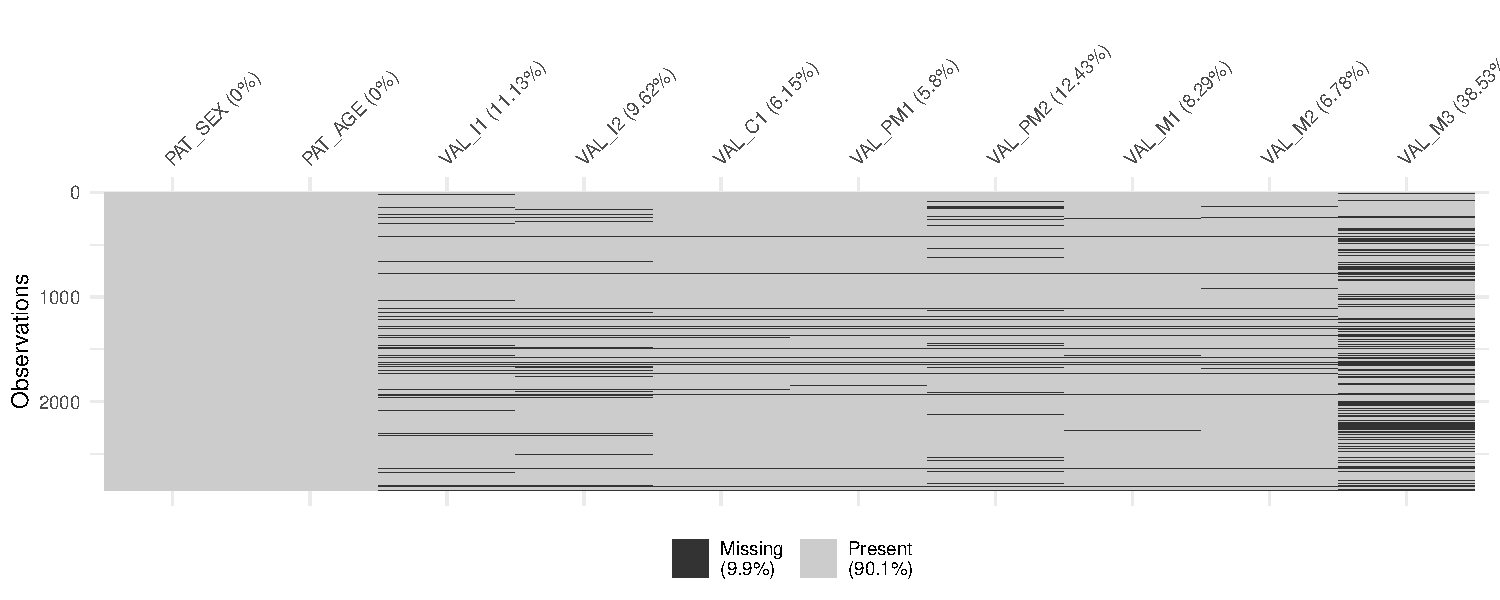
\includegraphics{paper_teeth_files/figure-latex/unnamed-chunk-3-1.pdf}

Nonetheless, because of the first reason of incompleteness we presented
(that teeth grow at different stages in life) we think that imputing
missing values makes sense, our approach is explained when we discuss
about our methodology.

\hypertarget{methodology}{%
\section{Methodology}\label{methodology}}

As predictive power is our main goal, we are interested in finding the
model that minimizes an error score on unseen data. The score we chose
is the Mean Absolute Error defined as
\(mae=(\frac{1}{n})\sum_{i=1}^{n}\left | y_{i} - x_{i} \right |\). \#\#
Ordinal encoding

\hypertarget{handling-missing-values}{%
\subsection{Handling missing values}\label{handling-missing-values}}

dependent \textcite{Kontopantelis2017}

\hypertarget{outlier-removal}{%
\subsection{Outlier removal}\label{outlier-removal}}

\hypertarget{model-developement}{%
\section{Model developement}\label{model-developement}}

\hypertarget{baseline-results-on-several-algorithms}{%
\subsection{Baseline results on several
algorithms}\label{baseline-results-on-several-algorithms}}

\hypertarget{results-on-best-tuned-gbrt}{%
\subsection{Results on best tuned
GBRT}\label{results-on-best-tuned-gbrt}}

\hypertarget{feature-importances}{%
\section{Feature importances}\label{feature-importances}}

\hypertarget{conclusion}{%
\section{Conclusion}\label{conclusion}}





\newpage
\singlespacing 
\printbibliography[title=References]

\end{document}
